\documentclass[compress]{beamer}
\usetheme{Antibes}
\usecolortheme{dolphin}
\usefonttheme[onlymath]{serif}

\usepackage{amsmath}
\usepackage{mathcomp}
\usepackage[utf8]{inputenc}
\usepackage{graphicx}
\graphicspath{{./images/}}
\usepackage{listings}
\usepackage{caption}
\usepackage{multirow}
\usepackage{url}
\usepackage[backend=biber,style=trad-abbrv]{biblatex}

\bibliography{literature}

\usepackage{tikz}
\usetikzlibrary{automata,positioning}

\title{Checking Equivalence of Nondeterministic Finite Automata}
\author{David Kofler}
\date{\today}
\institute{Master Seminar 2 \newline University of Innsbruck \newline Institute of Computer Science}


\begin{document}

\begin{frame}{}
	\maketitle
\end{frame}

\begin{frame}{}
	\tableofcontents
\end{frame}

\begin{frame}{Main Source}
  \fullcite{bonchi2013checking}
\end{frame}

\section{Introduction}



\begin{frame}{Applications}
  \begin{itemize}
    \item Model checking
    \item Compiler construction
    \item Testing microchips
    \item Homework/Exams: Did I/a student simplify a given automata correctly?
  \end{itemize}
\end{frame}

\begin{frame}{Complexity}
  \begin{itemize}
    \item For DFA: $\mathcal{O}(n + \alpha(n))$ algorithm by Hopcroft and Karp\\
          \fullcite{hopcroft1971linear}
    \item For NFA: $\mathcal{O}(2^n)$ (PSPACE-complete)
  \end{itemize}
\end{frame}

\begin{frame}{Example I}
  \begin{figure}
    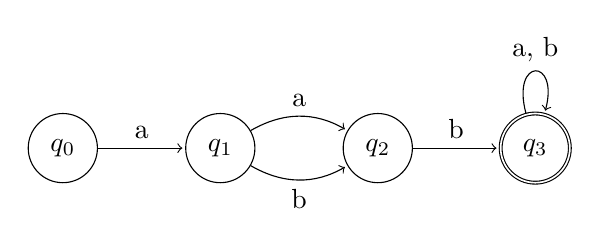
\begin{tikzpicture}[shorten >=1pt,node distance=2cm,on grid,auto]
      \node[state] (q_0) [] {$q_0$};
      \node[state] (q_1) [right=of q_0] {$q_1$};
      \node[state] (q_2) [right=of q_1] {$q_2$};
      \node[state,accepting] (q_3) [right=of q_2] {$q_3$};
        \path[->]
        (q_0) edge node {a} (q_1)
        (q_1) edge [bend left] node {a} (q_2)
              edge [bend right] node [below] {b} (q_2)
        (q_2) edge node {b} (q_3)
        (q_3) edge [loop above] node {a, b} ();
    \end{tikzpicture}
  \end{figure}
\end{frame}


\begin{frame}{Example II - i}
  \begin{figure}
    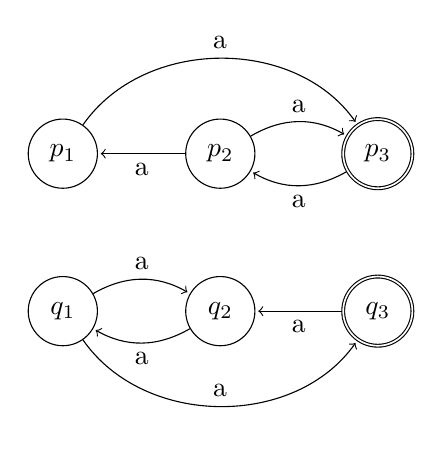
\begin{tikzpicture}[shorten >=1pt,node distance=2cm,on grid,auto]
      \node[state] (p_1) [] {$p_1$};
      \node[state] (p_2) [right=of p_1] {$p_2$};
      \node[state,accepting] (p_3) [right=of p_2] {$p_3$};
      \node[state] (q_1) [below=of p_1] {$q_1$};
      \node[state] (q_2) [right=of q_1] {$q_2$};
      \node[state,accepting] (q_3) [right=of q_2] {$q_3$};
        \path[->]
          (p_1) edge [bend left=55pt] node {a} (p_3)
          (p_2) edge [bend left] node {a} (p_3)
          (p_3) edge [bend left] node {a} (p_2)
          (p_2) edge node {a} (p_1)

          (q_1) edge [bend left] node {a} (q_2)
          (q_2) edge [bend left] node {a} (q_1)
          (q_1) edge [bend right=55pt] node {a} (q_3)
          (q_3) edge node {a} (q_2);
    \end{tikzpicture}
  \end{figure}
\end{frame}

\begin{frame}{Example II - ii}
  \begin{figure}
    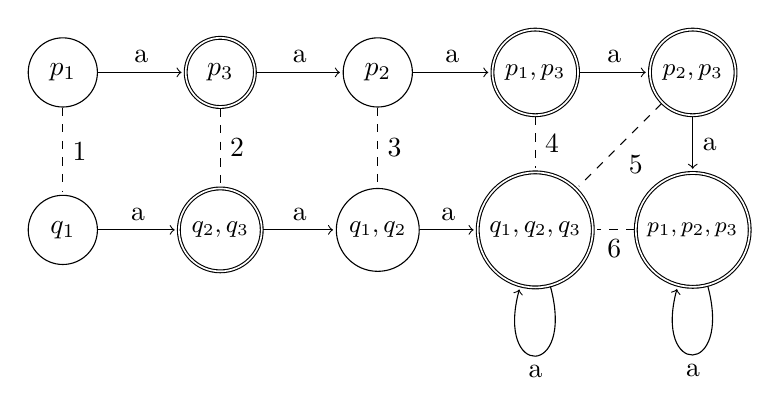
\begin{tikzpicture}[shorten >=1pt,node distance=2cm,on grid,auto]
      \node[state] (p_1) [] {$p_1$};
      \node[state,accepting] (p_3) [right=of p_1] {$p_3$};
      \node[state] (p_2) [right=of p_3] {$p_2$};
      \node[state,accepting] (p_13) [right=of p_2] {\small$p_1, p_3$};
      \node[state,accepting] (p_23) [right=of p_13] {\small$p_2, p_3$};
      \node[state,accepting] (p_123) [below=of p_23] {\footnotesize$p_1, p_2, p_3$};

      \node[state] (q_1) [below=of p_1] {$q_1$};
      \node[state,accepting] (q_23) [right=of q_1] {\small{$q_2, q_3$}};
      \node[state] (q_12) [right=of q_23] {\small$q_1, q_2$};
      \node[state,accepting] (q_123) [right=of q_12] {\small$q_1,q_2,q_3$};

      \path[dashed]
        (p_1) edge node {1} (q_1)
        (p_3) edge node {2} (q_23)
        (p_2) edge node {3} (q_12);
      \path[dashed]
        (p_13) edge node {4} (q_123)
        (p_23) edge node {5} (q_123)
        (p_123) edge node {6} (q_123);
      \path[->]
        (p_1) edge node {a} (p_3)
        (p_3) edge node {a} (p_2)
        (p_2) edge node {a} (p_13)
        (p_13) edge node {a} (p_23)
        (p_23) edge node {a} (p_123)
        (p_123) edge [loop below] node {a} ()

        (q_1) edge node {a} (q_23)
        (q_23) edge node {a} (q_12)
        (q_12) edge node {a} (q_123)
        (q_123) edge [loop below] node {a} ();
    \end{tikzpicture}
  \end{figure}
\end{frame}

\begin{frame}{Example II - ii}
  \begin{figure}
    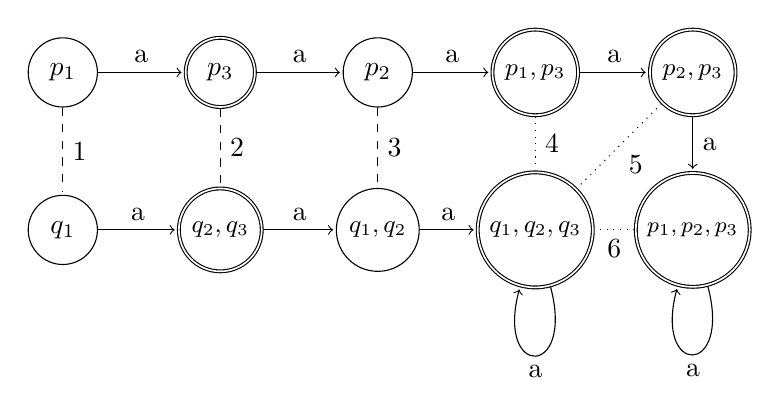
\begin{tikzpicture}[shorten >=1pt,node distance=2cm,on grid,auto]
      \node[state] (p_1) [] {$p_1$};
      \node[state,accepting] (p_3) [right=of p_1] {$p_3$};
      \node[state] (p_2) [right=of p_3] {$p_2$};
      \node[state,accepting] (p_13) [right=of p_2] {\small$p_1, p_3$};
      \node[state,accepting] (p_23) [right=of p_13] {\small$p_2, p_3$};
      \node[state,accepting] (p_123) [below=of p_23] {\footnotesize$p_1, p_2, p_3$};

      \node[state] (q_1) [below=of p_1] {$q_1$};
      \node[state,accepting] (q_23) [right=of q_1] {\small{$q_2, q_3$}};
      \node[state] (q_12) [right=of q_23] {\small$q_1, q_2$};
      \node[state,accepting] (q_123) [right=of q_12] {\small$q_1,q_2,q_3$};

      \path[dashed]
        (p_1) edge node {1} (q_1)
        (p_3) edge node {2} (q_23)
        (p_2) edge node {3} (q_12);
      \path[dotted]
        (p_13) edge node {4} (q_123)
        (p_23) edge node {5} (q_123)
        (p_123) edge node {6} (q_123);
      \path[->]
        (p_1) edge node {a} (p_3)
        (p_3) edge node {a} (p_2)
        (p_2) edge node {a} (p_13)
        (p_13) edge node {a} (p_23)
        (p_23) edge node {a} (p_123)
        (p_123) edge [loop below] node {a} ()

        (q_1) edge node {a} (q_23)
        (q_23) edge node {a} (q_12)
        (q_12) edge node {a} (q_123)
        (q_123) edge [loop below] node {a} ();
    \end{tikzpicture}
  \end{figure}
\end{frame}


\begin{frame}{Nondeterministic finite automata}
  \begin{block}{Definition}
    \begin{itemize}
      \item $N := (Q, \Sigma, o, \delta)$
      \item $Q$ and $\Sigma$ are finite sets
      \item $o : Q \to \{\emptyset, \{\epsilon\} \}$
      \item $\delta : Q \to \Sigma \to \mathcal{P}(Q)$
      \item $\mathcal{L} : Q \to \mathcal{P}(\Sigma^\ast)$
    \end{itemize}
  \end{block}
\end{frame}

\begin{frame}{Naive algorithm for checking equivalence}
  \begin{align*}
    \underline{Naive(p, q)}: &\quad Q \to Q \to \{true, false\} \\
    \text{(1) } & R := \emptyset, todo := \emptyset \\
    \text{(2) } & todo := todo \cup \{(p, q)\} \\
    \text{(3) } & \text{while } todo \neq \emptyset \text{ do}\\
      & \text{(3.1)}\quad todo := todo \setminus (p', q')\\
      & \textbf{(3.2)}\quad \textbf{if } \mathbf{(p', q') \in} \textbf{ R} \textbf{ then goto (3)}\\
      & \text{(3.3)}\quad \text{if } o(p') \neq o(q) \text{ then return } false\\
      & \text{(3.4)}\quad todo := todo \cup \bigcup_{a \in \Sigma}{(\delta(p', a), \delta(q', a))}\\
      & \text{(3.5)}\quad R := R \cup \{(p', q')\} \\
    \text{(4) } & \text{return } true\\
  \end{align*}
\end{frame}

\begin{frame}{Language equivalence of NFAs}
  \begin{block}{Bisimulations on sets of states}<1->
    \begin{itemize}
      \item Relation between sets of states: $R \subseteq \mathcal{P}(Q)^2$% \times \mathcal{P}(Q)$
      \item $R$ is bisimulation $\Leftrightarrow \forall Q_1, Q_2 \in \mathcal{P}(Q): $
        \begin{itemize}
          \item $o^\#(Q_1) = o^\#(Q_2)$, and
          \item $\forall a \in \Sigma: (\delta^\#(Q_1, a), \delta^\#(Q_2, a)) \in R$
        \end{itemize}
    \end{itemize}
  \end{block}

  \begin{block}{Language equivalence}<2->
    \begin{itemize}
      %\item $p \sim q \Leftrightarrow \mathcal{L}(\{p\}) = \mathcal{L}(\{q\})$
      \item
      Coinduction:\\
        $\mathcal{L}(P) = \mathcal{L}(Q) \Leftrightarrow \exists$ bisimulation $R: (P, Q) \in R$
    \end{itemize}
  \end{block}
\end{frame}

\begin{frame}{Determinisation by powerset construction}
  \begin{figure}
    \begin{align*}
      o^\#(Q) &= \bigcup_{q \in Q} o(q)\\
      \delta^\#(Q, a) &= \bigcup_{q \in Q} \delta(q, a)
      %o^\#(X) = &\begin{cases}
      %    o(x)                    &\text{ if } X = \{x\}, x \in S\\
      %    \emptyset               &\text{ if } X = \emptyset\\
      %    o^\#(X_1) \cup o^(X_2)  &\text{ if } X = X_1 \cup X_2\\
      %  \end{cases}\\
      %\delta^\#(X, a) = &\begin{cases}
      %    \delta(x, a)                              &\text{ if } X =\{x\}, x \in S\\
      %    \emptyset                                 &\text{ if } X = \emptyset\\
      %    \delta^\#(X_1, a) \cup \delta^\#(X_2, a)  &\text{ if } X = X_1 \cup X_2\\
      %  \end{cases}
    \end{align*}
  \end{figure}

  \begin{block}{Determinised NFA}<2->
    We obtain the determinised automaton $N^\# = (\mathcal{P}(S), \Sigma, o^{\#}, d^{\#})$
      from the NFA $N = (S, \Sigma, o, \delta)$
  \end{block}
\end{frame}

\begin{frame}{Contribution of Pous et Bonchi}
  \begin{itemize}
      \item<1-> $\textbf{(3.2)}\quad \textbf{if } \mathbf{(p', q') \in} \textbf{ R} \textbf{ then goto (3)}$
      \item<2-> $(p', q') \in R$ can be replaced by $(p', q') \in f(R)$
      \item<2-> $f$ has to be \textbf{compatible}
      \item<3-> Existing algorithms differ only by $f$
      \item<4-> There is a very effective choice of $f$ for NFAs
    \end{itemize}
\end{frame}

\begin{frame}{Compatible functions}
  \begin{itemize}
    \item<1-> Identity function
    \item<2-> Symmetric closure: $(q, p) \in R \Rightarrow (p, q) \in R$
    \item<3-> Equivalence closure:
      \begin{align*}
        \forall p: (p, p) \in R\\
        (p, q) \in R \Rightarrow (q, p) \in R\\
        (p, q) \in R \land (q, r) \in R \Rightarrow (p, r) \in R\\
      \end{align*}
    \item<4-> Congruence closure (for determinised NFAs):\\
        $(P_1, Q_1) \in R \land (P_2, Q_2) \in R \Rightarrow (P_1 \cup Q_2, P_2 \cup Q_2) \in R$
  \end{itemize}
\end{frame}

\begin{frame}{Data structure for congruence closure}
  \begin{block}{Hello}
    \begin{itemize}
        \item Binary decision diagrams
        \item Pous and Bonchi's approach: Set rewriting
        \item $(P, Q) \in c(R) \Leftrightarrow P \downarrow_R = Q \downarrow_R$
    \end{itemize}
  \end{block}
  \begin{figure}
    %\begin{table}[]
%\centering
%\caption{My caption}
%\label{my-label}
$ R = \{ (\{p\}, \{r\}), (\{q, s\}, \{r\}) \}$
\begin{tabular}{ccccccccc}
$\{p, q\}$ &            &               &            &                  &            &            &            & $\{r\}$ \\
           & $\searrow$ &               &            &                  &            &            & $\swarrow$ &         \\
           &            & $\{p, q, r\}$ &            &                  &            & $\{p, r\}$ &            &         \\
           &            &               & $\searrow$ &                  & $\swarrow$ &            &            &         \\
           &            &               &            & $\{p, q, r, s\}$ &            &            &            &
\end{tabular}
%\end{table}

  \end{figure}
\end{frame}

\begin{frame}{Set rewriting}
  \begin{itemize}
    \item Store only processed pairs and their normal forms
    \item View $R$ as set of rewrite rules:
      \begin{align*}
        \forall (P, Q) \in R: \quad&P \rightsquigarrow P \cup Q\\
                              &Q \rightsquigarrow P \cup Q\\
        \forall Q: P \rightsquigarrow P' \Rightarrow & P \cup Q \rightsquigarrow P' \cup Q
      \end{align*}
  \end{itemize}
\end{frame}

\begin{frame}{Compatibility}
  \begin{block}{Progression}
    \begin{itemize}
      %\item $R, R' \subseteq S \times S$
      \item $R \rightarrowtail R' \Leftrightarrow \forall (x, y) \in R:$\\
        \begin{itemize}
          \item $o(x) = o(y)$, and
          \item $\forall a \in \Sigma: (\delta(x, a), \delta(y, a)) \in R'$
        \end{itemize}
      %\item $R \rightarrowtail R \Leftrightarrow R \text{ is bisimulation}$
    \end{itemize}
  \end{block}

  \begin{block}{Compatibility}
    $f : (S \times S) \to (S \times S)$ is compatible iff \\
    \begin{itemize}
      \item $f$ monotone: $\forall R: R \subseteq f(R)$, and
      \item $f$ preserves $\rightarrowtail$:
        $R \rightarrowtail R' \Rightarrow f(R) \rightarrowtail f(R')$
    \end{itemize}
  \end{block}
\end{frame}

\section{Experimental Results}

\begin{frame}{Language equivalence - 50 states}
  \begin{figure}
    % Please add the following required packages to your document preamble:
% \usepackage{multirow}
%\begin{table}[]
%\centering
%\caption{My caption}
%\label{my-label}
\begin{tabular}{l|rrrr|rrrr}
\multirow{2}{*}{} & \multicolumn{4}{l|}{Required time {[}ms{]}} & \multicolumn{4}{l}{Processed pairs} \\ \cline{2-9}
                  & 50\% & 90\% & 99\% & 100\%                 & 50\%   & 90\%   & 99\%    & 100\%   \\ \hline
HK                & 7    & 22   & 50   & 119                   & 2511   & 6299   & 12.5k   & 25.2k   \\
AC                & 2    & 3    & 142  & 1083                  & 112    & 245    & 2130    & 5208    \\
HKC               & 0    & 0    & 0    & 0                     & 21     & 26     & 32      & 63      \\
%AC'               & 2    & 2    & 38   & 211                   & 79     & 131    & 1098    & 1926    \\
%HKC'              & 0    & 0    & 0    & 0                     & 18     & 23     & 28      & 58
\end{tabular}
%\end{table}

  \end{figure}
\end{frame}

\begin{frame}{Language equivalence - 100 states}
  \begin{figure}
    % Please add the following required packages to your document preamble:
% \usepackage{multirow}
%\begin{table}[]
%\centering
%\caption{My caption}
%\label{my-label}
\begin{tabular}{l|llll|llll}
\multirow{2}{*}{} & \multicolumn{4}{l|}{Required time {[}s{]}} & \multicolumn{4}{l}{Processed pairs} \\ \cline{2-9}
                  & 50\%     & 90\%      & 99\%     & 100\%    & 50\%    & 90\%   & 99\%    & 100\%  \\ \hline
HK                & 0.373    & 1.207     & 3.435    & 5.660    & 10.4k   & 28k    & 58.7k   & 87k    \\
AC                & 0.003    & 0.004     & 3.214    & 36.99    & 204     & 298    & 13.8k   & 48k    \\
HKC               & 0.000    & 0.000     & 0.000    & 0.001    & 36      & 44     & 54      & 70     \\
AC'               & 0.003    & 0.004     & 0.738    & 6.966    & 152     & 211    & 4087    & 18.4k  \\
HKC'              & 0.000    & 0.000     & 0.000    & 0.001    & 31      & 39     & 46      & 64
\end{tabular}
%\end{table}

  \end{figure}
\end{frame}

\begin{frame}{Language equivalence - 1000 states}
  \begin{figure}
    % Please add the following required packages to your document preamble:
% \usepackage{multirow}
%\begin{table}[]
%\centering
%\caption{My caption}
%\label{my-label}
\begin{tabular}{l|llll|llll}
\multirow{2}{*}{} & \multicolumn{4}{l|}{Required time {[}s{]}} & \multicolumn{4}{l}{Processed pairs} \\ \cline{2-9}
                  & 50\%     & 90\%     & 99\%    & 100\%      & 50\%   & 90\%   & 99\%  & 100\%     \\ \hline
AC                & 0.029    & 0.031    & 0.038   & $\infty$   & 1808   & 1878   & 2282  & $\infty$  \\
HKC               & 0.007    & 0.022    & 0.055   & 0.093      & 228    & 271    & 304   & 337       \\
AC'               & 0.074    & 0.080    & 0.092   & $\infty$   & 1409   & 1488   & 1674  & $\infty$  \\
HKC'              & 0.008    & 0.019    & 0.041   & 0.077      & 202    & 238    & 265   & 299
\end{tabular}
%\end{table}

  \end{figure}
\end{frame}

\begin{frame}{Language inclusion - Matches}
  \begin{figure}
    % Please add the following required packages to your document preamble:
% \usepackage{multirow}
%\begin{table}[]
%\centering
%\caption{My caption}
%\label{my-label}
\begin{tabular}{l|llll|}
\multirow{2}{*}{} & \multicolumn{4}{l|}{Inclusions (564 pairs)} \\ \cline{2-5}
                  & 50\%      & 90\%      & 99\%     & 100\%    \\ \hline
AC                & 0.036     & 0.860     & 4.981    & 5.084    \\
HKC               & 0.049     & 0.798     & 6.494    & 6.762    \\
AC'               & 0.013     & 0.167     & 1.326    & 1.480    \\
HKC'              & 0.000     & 0.034     & 0.224    & 0.345
\end{tabular}
%\end{table}

  \end{figure}
\end{frame}

\begin{frame}{Language inclusion - Mismatches}
  \begin{figure}
    % Please add the following required packages to your document preamble:
% \usepackage{multirow}
%\begin{table}[]
%\centering
%\caption{My caption}
%\label{my-label}
\begin{tabular}{l|llll}
\multirow{2}{*}{} & \multicolumn{4}{c}{Counterexamples (518 pairs) {[}ms{]}} \\ \cline{2-5}
                  & 50\% & 90\%  & 99\%  & 100\%     \\ \hline
AC                & 9    & 94    & 1412  & 2887     \\
HKC               & 0    & 14    & 916   & 2685     \\
%AC'               & 12   & 107   & 1047  & 1134     \\
%HKC'              & 1    & 5     & 25    & 383
\end{tabular}
%\end{table}

  \end{figure}
\end{frame}

\section{Conclusion}

\begin{frame}{Main Takeaways}
  \begin{itemize}
    \item<1-> Naive algorithm, ACs, HK, HKC, and other variants can be uniformely
      presented by using coinductive techniques
    \item<2-> The AC algorithms perform surprisingly bad
      \begin{itemize}
        \item Maybe it is unfair to let \textbf{libvata} operate solely on string automata?
      \end{itemize}
  \end{itemize}
\end{frame}

\begin{frame}
  \begin{center}
    \huge{Questions \& Discussion}
  \end{center}
\end{frame}

\end{document}
